%!TEX root=../../main.tex

%_______________
\section{Exercises}

%_______________
\subsection{Random variables}

% 1 (oi_biostat)

\eoce{\qt{Gull clutch size\label{gull_eggs}}
	Large black-tailed gulls usually lay one to three eggs, and rarely have a fourth egg clutch. It is thought that clutch sizes are effectively limited by how effectively parents can incubate their eggs. Suppose that on average, gulls have a 25\% of laying 1 egg, 40\% of laying 2 eggs, 30\% chance of laying 3 eggs, and 5\% chance of laying 4 eggs.
	\begin{parts}
		\item Calculate the expected number of eggs laid by a random sample of 100 gulls. 
		\item Calculate the standard deviation of the number of eggs laid by a random sample of 100 gulls.
	\end{parts}	
}{}

% scenario from incubation_capacity

% 2, oi_edited (from ch. 2)

\eoce{\qt{Hearts win\label{hearts}} In a card game, the player starts with a well-
	shuffled full deck and draw 3 cards without replacement. If the player draw 3 hearts, 
	they win \$50. If they draw 3 black cards, they win \$25. For any other draws, nothing is won.
	
	\begin{parts}
		\item Create a probability model for the amount of money that can be won playing this game, and find the expected winnings. Also, compute the standard deviation of this distribution.
		\item If the game costs \$5 to play, what would be the expected value and 
		standard deviation of the net profit (or loss)? 
		\item If the game costs \$5 to play, is it advantageous to play this game? Explain.
	\end{parts}
}{}

% 3

\eoce{\qt{Baggage fees\label{baggage_fees}} An airline charges the following 
	baggage fees: \$25 for the first bag and \$35 for the second. Suppose 54\% of 
	passengers have no checked luggage, 34\% have one piece of checked luggage and 
	12\% have two pieces. Suppose that a negligible portion of people check more than 
	two bags.
	\begin{parts}
		\item Build a probability model, compute the average revenue per passenger, and 
		compute the corresponding standard deviation.
		\item About how much revenue should the airline expect for a flight of 120 
		passengers? With what standard deviation? Note any assumptions made and whether they are justified.
	\end{parts}
}{}

% 4

\eoce{\qt{Scooping ice cream\label{scoop_ice_cream}} Ice cream usually comes in 1.5 quart boxes (48 fluid ounces), and ice cream scoops hold about 2 ounces. 
	However, there is some variability in the amount of ice cream in a box as well as 
	the amount of ice cream scooped out. We represent the amount of ice cream in the 
	box as $X$ and the amount scooped out as $Y$. Suppose these random variables have 
	the following means, standard deviations, and variances:
	\begin{center}
		\begin{tabular}{l ccc}
			\hline
			& mean & SD & variance \\
			\hline
			$X$ & 48       & 1      & 1     \\
			$Y$ & 2    & 0.25   & 0.0625    \\
			\hline
		\end{tabular}
	\end{center}
	\begin{parts}
		\item An entire box of ice cream, plus 3 scoops from a second box is served at a 
		party. How much ice cream do you expect to have been served at this party? What 
		is the standard deviation of the amount of ice cream served?
		\item How much ice cream would you expect to be left in the box after scooping 
		out one scoop of ice cream? That is, find the expected value of $X-Y$. What is 
		the standard deviation of the amount left in the box?
		\item Using the context of this exercise, explain why we add variances when we 
		subtract one random variable from another.
	\end{parts}
}{}


%_______________
\subsection{Binomial distribution}

% 5, edited

\eoce{\qt{Underage drinking, Part I\label{underage_drinking_intro}} Data collected 
	by the Substance Abuse and Mental Health Services Administration (SAMSHA) 
	suggests that 69.7\% of 18-20 year olds consumed alcoholic beverages in 2008.
	\footfullcite{webpage:alcohol}
	\begin{parts}
		\item Suppose a random sample of ten 18-20 year olds in the US is taken. Is the use 
		of the binomial distribution appropriate for calculating the probability that 
		exactly six consumed alcoholic beverages? Explain.
		\item Calculate the probability that exactly 6 out of 10 randomly sampled 18-
		20 year olds consumed an alcoholic drink.
		\item What is the probability that exactly four out of the ten 18-20 year 
		olds have \textit{not} consumed an alcoholic beverage?
		\item What is the probability that at most 2 out of 5 randomly sampled 18-20 
		year olds have consumed alcoholic beverages?
		\item What is the probability that at least 1 out of 5 randomly sampled 18-20 
		year olds have consumed alcoholic beverages?
	\end{parts}
}{}

% 6, edited

\eoce{\qt{Chickenpox, Part I\label{chicken_pox_intro}} The National Vaccine 
	Information Center estimates that 90\% of Americans have had chickenpox by 
	the time they reach adulthood.  \footfullcite{webpage:chickenpox}
	\begin{parts}
		\item Suppose we take a random sample of 100 American adults. Is the use of 
		the binomial distribution appropriate for calculating the probability that 
		exactly 97 had chickenpox during childhood? Explain.
		\item Calculate the probability that exactly 97 out of 100 randomly sampled 
		American adults had chickenpox during childhood.
		\item What is the probability that exactly 3 out of a new sample of 100 
		American adults have \textit{not} had chickenpox in their childhood?
		\item What is the probability that at least 1 out of 10 randomly sampled 
		American adults have not had chickenpox?
		\item What is the probability that at most 7 out of 10 randomly sampled 
		American adults have had chickenpox?
	\end{parts}
}{}

% 7 (oi_biostat)

\eoce{\qt{Donating blood\label{abo_blood}}
When patients receive blood transfusions, it is critical that the blood type of the donor is compatible with the patients, or else an immune system response will be triggered. For example, a patient with Type O- blood can only receive Type O- blood, but a patient with Type O+ blood can receive either Type O+ or Type O-. Furthermore, if a blood donor and recipient are of the same ethnic background, the chance of an adverse reaction may be reduced. According to a 10-year donor database, 0.37 of white, non-Hispanic donors are O+ and 0.08 are O-. 
\begin{parts}
\item Consider a random sample of 15 white, non-Hispanic donors. Calculate the expected value of individuals who could be a donor to a patient with Type O+ blood. With what standard deviation?
\item What is the probability that 3 or more of the people in this sample could donate blood to a patient with Type O- blood?
\end{parts}	
}{}

% from abo_blood

% 8 (oi biostat)

\eoce{\qt{Hepatitis C\label{hepatitis_c}}
Hepatitis C is spread primarily through contact with the blood of an infected person, and is nearly always transmitted through needle sharing among intravenous drug users. Suppose that in a month's time, an IV drug user has a 30\% chance of contracting hepatitis C through needle sharing. What is the probability that 3 out of 5 IV drug users contract hepatitis C in a month? Assume that the drug users live in different parts of the country.	
}{}

% from midterm (2016), question 1c


% 9 (oi_biostat)

\eoce{\qt{Wolbachia infection\label{wolbachia_infection}}
Approximately 12,500 stocks of \textit{Drosophila melanogaster} flies are kept at The Bloomington \textit{Drosophila} Stock Center for research purposes. A 2006 study examined how many stocks were infected with Wolbachia, an intracellular microbe that can manipulate host reproduction for its own benefit. About 30\% of stocks were identified as infected. Researchers working with infected stocks should be cautious of the potential confounding effects that Wolbachia infection may have on experiments. Consider a random sample of 250 stocks.
\begin{parts}
\item Calculate the probability that exactly 60 stocks are infected.
\item Calculate the probability that at most 60 stocks are infected.
\item Calculate the probability that at least 80 stocks are infected.
\item If a researcher wants to make sure that no more than 40\% of the stocks used for an experiment are infected, does it seem reasonable to take a random sample of 250?
\end{parts}
}{}

% from wolbachia_prevalence

% 10 

\eoce{\qt{Eye color, Part I\label{eye_color_binomial}} Suppose that two parents with brown eyes carry genes that make it possible for their children to have brown eyes (probability 0.75), blue eyes (0.125), or green eyes (0.125). 
	\begin{parts}
		\item What is the probability that their first child will have green eyes and 
		the second will not?
		\item What is the probability that exactly one of their two children will 
		have green eyes?
		\item If they have six children, what is the probability that exactly two 
		will have green eyes?
		\item If they have six children, what is the probability that at least one 
		will have green eyes?
	\end{parts}
}{}

% 11 (oi_biostat)

\eoce{\qt{Hyponatremia\label{hyponatremia}}
Hyponatremia (low sodium levels) occurs in a certain proportion of marathon runners during a race. Suppose that historically, the proportion of runners who develop hyponatremia is 0.12. In a certain marathon, there are 200 runners participating.	
\begin{parts}
\item How many cases of hyponatremia are expected during the marathon?
\item What is the probability of more than 30 cases of hyponatremia occurring?
\end{parts}	
}{}

% from unit 3 lecture (2016), slide 26

%_______________
\subsection{Normal distribution}

% 12 

\eoce{\qt{Area under the curve, Part I\label{area_under_curve_1}} What percent of a 
	standard normal distribution $N(\mu=0, \sigma=1)$ is found in each region? 
	Be sure to draw a graph. \vspace{-3mm}
	\begin{multicols}{4}
		\begin{parts}
			\item $Z < -1.35$
			\item $Z > 1.48$
			\item $-0.4 < Z < 1.5$
			\item $|Z| > 2$
		\end{parts}
	\end{multicols}
}{}

% 13 (oi_biostat)

\eoce{\qt{The standard normal distribution\label{standard_normal}}
	Consider the standard normal distribution with mean $\mu = 0$ and standard deviation $\sigma=1$. 
	\begin{parts}
		\item What is the probability that an outcome $Z$ is greater than 2.60?
		\item What is the probability that $Z$ is less than 1.35?
		\item What is the probability that $Z$ is between -1.70 and 3.10?
		\item What value of $Z$ cuts off the upper 15\% of the distribution?
		\item What value of $Z$ marks off the lower 20\% of the distribution?
	\end{parts}
}{}

% from pset 3 (2016), problem 7


% 14 oi, edited

\eoce{\qt{GRE scores\label{GRE_intro}} The Graduate Record Examination (GRE) is a standardized test commonly taken by graduate school applicants in the United States. The total score is comprised of three components: Quantitative Reasoning, Verbal Reasoning, and Analytical Writing. The first two components are scored from 130 - 170. The mean score for Verbal Reasoning section for all test takers was 151 with a standard deviation of 7, and the mean score for the Quantitative Reasoning was 153 with a standard deviation of 7.67. Suppose that both distributions are nearly normal. 
	\begin{parts}
		\item A student scores 160 on the Verbal Reasoning section and 157 on the Quantitative Reasoning section. Relative to the scores of other students, which section did the student perform better on?
		\item Calculate the student's percentile scores for the two sections. What percent of test takers performed better on the Verbal Reasoning section?
		\item Compute the score of a student who scored in the 80$^{th}$ percentile on the Quantitative Reasoning section.
		\item Compute the score of a student who scored worse than 70\% of the test takers on the Verbal Reasoning section.
	\end{parts}
}{}

% 15 oi, edited

\eoce{\qt{Triathlon times\label{triathlon_times}}
	In triathlons, it is common for racers to be placed into age and gender groups. The finishing times of men ages 30-34 has mean of 4,313 seconds with a standard deviation of 583 seconds. The finishing times of the women ages 25-29 has a mean of 5,261 seconds with a standard deviation of 807 seconds. The distribution of finishing times for both groups is approximately normal. Note that a better performance corresponds to a faster finish.
	\begin{parts}
		\item If a man of the 30-34 age group finishes the race in 4,948 seconds, what percent of the triathletes in the group did he finish faster than?
		\item If a woman of the 25-29 age group finishes the race in 5,513 seconds, what percent of the triathletes in the group did she finish faster than?
		\item Calculate the cutoff time for the fastest 5\% of athletes in the men's group.
		\item Calculate the cutoff time for the slowest 10\% of athletes in the women's group.	
	\end{parts}
}{}

% 16 (oi_biostat)

\eoce{\qt{Osteoporosis\label{osteoporosis}}
	The World Health Organization defines osteoporosis in young adults as a measured bone mineral density 2.5 or more standard deviations below the mean for young adults. Assume that bone mineral density follows a normal distribution in young adults. What percentage of young adults suffer from osteoporosis according to this criterion?	
}{}

% from pset 3 (2016), problem 8

% 17

\eoce{\qt{LA weather\label{la_weather_intro}} The average daily high 
	temperature in June in LA is 77\degree F with a standard deviation of 
	5\degree F. Suppose that the temperatures in June closely follow a normal 
	distribution. 
	\begin{parts}
		\item What is the probability of observing an 83\degree F temperature or 
		higher in LA during a randomly chosen day in June?
		\item How cold are the coldest 10\% of the days during June in LA?
	\end{parts}
}{}

% 18 (oi_biostat)

\eoce{\qt{Clutch volume\label{clutch volume}}
	A study investigating maternal investment in a frog species found on the Tibetan Plateau reported data on the volume of egg clutches measured across 11 study sites. The distribution is roughly normal, with approximate distribution $N(882.5, 380) \ mm^{3}$.
	\begin{parts}
		\item What is the probability of observing an egg clutch between volume 700-800 $mm^{3}$?
		\item How large are the largest 5\% of egg clutches?
	\end{parts}	
}{}

% from clutch volume

% 19 (oi biostat)

\eoce{\qt{Glucose levels\label{glucose_levels}}
	Fasting blood glucose levels for normal non-diabetic individuals are normally distributed in the population, with mean $\mu = 85$ mg/dL and standard deviation $\sigma = 7.5$ mg/dL. 
	\begin{parts}
		\item What is the probability that a randomly chosen member of the population has a fasting glucose level higher than 100 mg/dL?
		\item  What value of fasting glucose level defines the lower $5^{th}$ percentile of the distribution?	
	\end{parts}	
}{}

% from midterm (2016), problem 1a

% 20 (oi biostat)

\eoce{\qt{Arsenic poisoning\label{arsenic}}
	Arsenic blood concentration is normally distributed with mean $\mu = 3.2$ $\mu$g/dl and standard deviation $\sigma = 1.5$ $\mu$g/dl. What range of arsenic blood concentration defines the middle 95\% of this distribution?
}{}

% from pset 3 (2016), problem 9

% 21 (oi_biostat)
\eoce{\qt{Age at childbirth\label{age_childbirth}}
	In the last decade, the average age of a mother at childbirth is 26.4 years, with standard deviation 5.8 years. The distribution of age at childbirth is approximately normal.
	\begin{parts}
		\item What proportion of women who give birth are 21 years of age or older?
		\item Giving birth at what age puts a woman in the upper 2.5\% of the age distribution?
	\end{parts}
}{}

% from unit 3 lecture slides (2016), slide 11

% 22

\eoce{\qt{Find the SD\label{find_sd}} Find the standard deviation of the 
	distribution in the following situations.
	\begin{parts}
		\item  MENSA is an organization whose members have IQs in the top 2\% of the 
		population. IQs are normally distributed with mean 100, and the minimum IQ 
		score required for admission to MENSA is 132.
		\item Cholesterol levels for women aged 20 to 34 follow an approximately 
		normal distribution with mean 185 milligrams per deciliter (mg/dl). Women 
		with cholesterol levels above 220 mg/dl are considered to have high 
		cholesterol and about 18.5\% of women fall into this category.
	\end{parts}
}{}

% 23

\eoce{\qt{SAT scores\label{sat_scores}} SAT scores (out of 2400) are distributed 
	normally with a mean of 1500 and a standard deviation of 300. Suppose a 
	school council awards a certificate of excellence to all students who score 
	at least 1900 on the SAT, and suppose we pick one of the recognized students 
	at random. What is the probability this student's score will be at least 
	2100? (The material covered in Section~\ref{conditionalProbabilitySection} 
	would be useful for this question.)
}{}

% 24, edited

\eoce{\qt{Underage drinking, Part II\label{underage_drinking_normal_approx}} As first referenced in Exercise~\ref{underage_drinking_intro}, about 70\% of 18-20 year olds consumed alcoholic beverages in 2008. Consider a random sample of fifty 18-20 year olds.
	\begin{parts}
		\item Of these fifty people, how many would be expected to have consumed alcoholic beverages? With what standard deviation?
		\item Evaluate the conditions for using the normal approximation to the binomial. What is the probability that 45 or more people in this sample have 
		consumed alcoholic beverages?
	\end{parts}
}{}

% 25, edited

\eoce{\qt{Chickenpox, Part II\label{chicken_pox_normal_approx}} As first referenced in Exercise~\ref{chicken_pox_intro}, about 90\% of American adults had chickenpox before adulthood. Consider a random sample of 120 American adults.
	\begin{parts}
		\item How many people in this sample would be expected to have had chickenpox 
		in their childhood? With what standard deviation?
		\item Evaluate the conditions for using the normal approximation to the binomial. What is the probability that 105 or fewer people in this sample have 
		had chickenpox in their childhood?
	\end{parts}
}{}

% 26

\eoce{\qt{University admissions\label{university_admissions}} Suppose a university 
	announced that it admitted 2,500 students for the following year's freshman 
	class. However, the university has dorm room spots for only 1,786 freshman 
	students. If there is a 70\% chance that an admitted student will decide to 
	accept the offer and attend this university, what is the approximate 
	probability that the university will not have enough dormitory room spots for 
	the freshman class?
}{}	
	
	
% 27, edited

\eoce{\qt{Heights of female college students\label{college_fem_heights}} The heights of 25 female college students are plotted below. Do these data appear to follow a normal distribution? Explain your reasoning.
		\begin{center}
			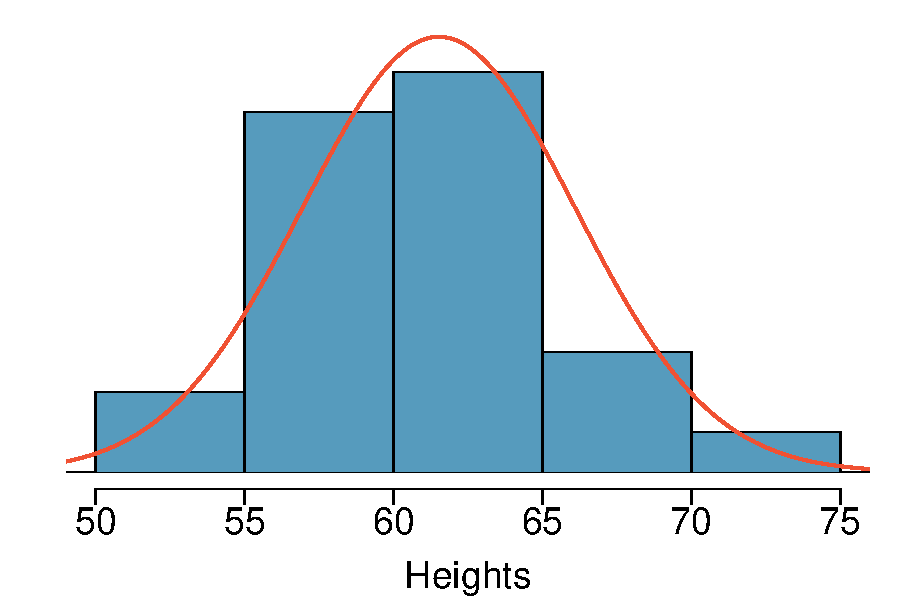
\includegraphics[width= 0.46\textwidth]{ch_distributions_oi_biostat/figures/eoce/college_fem_heights/college_fem_heights_hist.pdf}\ \ \ \ 
			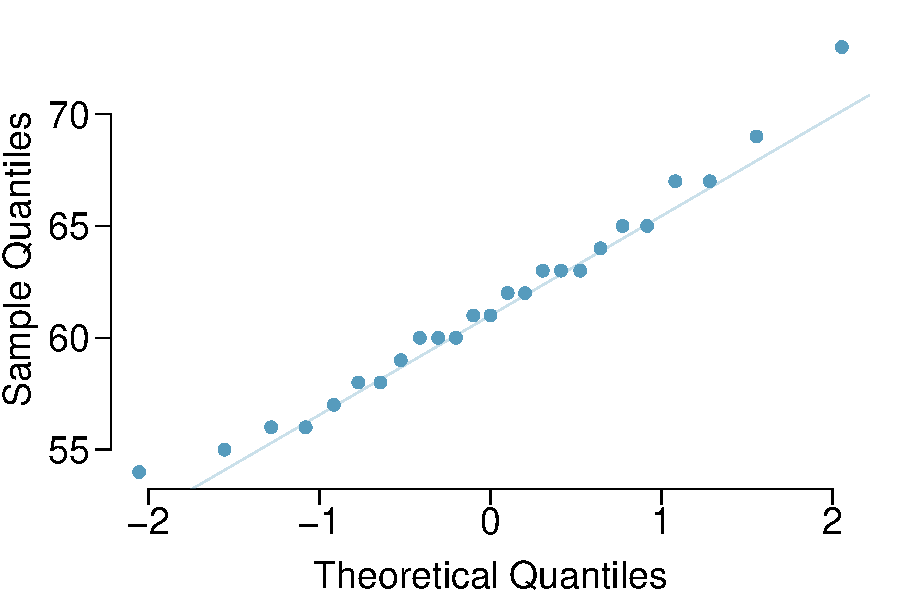
\includegraphics[width= 0.46\textwidth]{ch_distributions_oi_biostat/figures/eoce/college_fem_heights/college_fem_heights_qq.pdf}
		\end{center}
}{}


%_______________
\subsection{Poisson distribution}

% 28 (oi_biostat)

\eoce{\qt{Computing Poisson probabilities\label{computing_poisson}}
This is a simple exercise in computing probabilities for a Poisson random variable. Suppose that $X$ is a Poisson random variable with rate parameter $\lambda = 2$.	Calculate $P(X = 2)$, $P(X \leq 2)$, and $P(X \geq 3)$. 
}{}

% 29 oi, edited

\eoce{\qt{Stenographer's typos\label{stenographer_typos}} A very skilled 
	court stenographer makes one typographical error (typo) per hour on average.
	\begin{parts}
		\item What are the mean and the standard deviation of the number of typos 
		this stenographer makes in an hour?
		\item Calculate the probability that this stenographer makes at most 3 typos 
		in a given hour.
		\item Calculate the probability that this stenographer makes at least 5 typos over 3 hours.
	\end{parts}
}{}

% 30 (oi_biostat)

\eoce{\qt{Osteosarcoma in NYC\label{osteosarcoma_nyc}}
Osteosarcoma is a relatively rare type of bone cancer. It occurs most often in young adults, age 10-19: it is diagnosed in approximately 8 per 1,000,000 individuals per year in that age group. In New York City (including all five boroughs), the number of young adults in this age range is approximately 1,400,000.
\begin{parts}	
\item What is the expected number of cases of osteosarcoma in NYC in a given year?
\item What is the probability that 15 or more cases will be diagnosed in a given year?
\item The largest concentration of young adults in NYC is in the borough of Brooklyn, where the population in that age range is approximately 450,000. What is the probability of 10 or more cases in Brooklyn in a given year?	
\end{parts}
}{}

% from pset 3 (2016), problem 6

\noindent
\textit{Note: The following two problems are best done using statistical computing software.} \\

% 31 (oi_biostat)

\eoce{\qt{Hemophilia\label{hemophilia}}
	Hemophilia is a sex-linked bleeding disorder that slows the blood clotting process. In severe cases of hemophilia, continued bleeding occurs after minor trauma or even in the absence of injury. Hemophilia affects 1 in 5,000 male births. In the United States, about 400 males are born with hemophilia each year; there are approximately 4,000,000 births per year.
	\begin{parts}
		\item What is the probability that at most 380 newborns in a year are born with hemophilia?
		\item What is the probability that 450 or more newborns in a year are born with hemophilia?
		\item Consider a hypothetical country in which there are approximately 1.5 million births per year. If the incidence rate of hemophilia is equal to that in the US, how many newborns are expected to have hemophilia in a year, with what standard deviation?
	\end{parts}	
}{}

% from http://www.cdc.gov/ncbddd/hemophilia/data.html
% from http://www.cdc.gov/nchs/fastats/births.htm

% 32 (oi_biostat)

\eoce{\qt{Opioid overdose\label{opioid_overdose}}
The US Centers for Disease Control (CDC) has been monitoring the rate of deaths from opioid overdoses for at least the last 15 years. In 2013, the rate of opioid-related deaths has risen to 6.8 deaths per year per 100,000 non-Hispanic white members. In 2014-2015, the population of Essex County, MA, was approximately 769,000, of whom 73\% are non-Hispanic white. Assume that incidence rate of opioid deaths in Essex County is the same as the 2013 national rate. 
\begin{parts}
\item In 2014, Essex County reported 146 overdose fatalities from opioids. Assume that all of these deaths occurred in the non-Hispanic white members of the population. What is the probability of 146 or more such events a year?
\item What was the observed rate of opioid-related deaths in Essex County in 2014, stated in terms of deaths per 100,000 non-Hispanic white members of the population?
\item In 2015, Essex County reported 165 opioid-related deaths in its non-Hispanic white population. Using the rate from part (b), calculate the probability of 165 or more such events.
\end{parts}	
}{}

% from midterm (2016), question 3

%_______________
\subsection{Distributions related to Bernoulli trials}

%%geometric distribution

% 33

\eoce{\qt{Married women} \label{married_women} The 2010 American Community Survey 
estimates that 47.1\% of women ages 15 years and over are married. Suppose that a random sample of women in this age group are selected for a research study.
\footfullcite{marWomenACS}
\begin{parts}
\item On average, how many women would need to be sampled in order to select 
a married woman? What is the standard deviation?
\item If the proportion of married women were actually 30\%, what would be the new mean and standard deviation?
\item Based on the answers to parts (a) and (b), how does decreasing the 
probability of an event affect the mean and standard deviation of the wait time until success?
\end{parts}
}{}

% 34 (oi_biostat)

\eoce{\qt{Donating blood, Part II\label{abo_blood_geometric}} Recall from Problem~\ref{abo_blood} that a patient with Type O+ blood can receive either Type O+ or Type O- blood, while a patient with Type O- blood can only receive Type O- blood. According to data collected from blood donors, 0.37 of white, non-Hispanic donors are Type O+ and 0.08 are Type O-. For the following questions, assume that only white, non-Hispanic donors are being tested.
\begin{parts}
\item On average, how many donors would need to be randomly sampled for a Type O+ donor to be identified? With what standard deviation?
\item What is the probability that 4 donors must be sampled to identify a Type O+ donor?
\item What is the probability that more than 4 donors must be sampled to identify a Type O+ donor?
\item What is the probability of the first Type O- donor being found within the first 4 people?
\item On average, how many donors would need to be randomly sampled for a Type O- donor to be identified? With what standard deviation?
\item What is the probability that fewer than 4 donors must be tested before a Type O- donor is found?
\end{parts}	
}{}

% from abo_blood

% 35 (oi_biostat)

\eoce{\qt{Wolbachia infection, Part II\label{wolbachia_infection_geometric}} Recall from Problem~\ref{wolbachia_infection} that 30\% of the \textit{Drosophila} stocks at the BDSC are infected with Wolbachia. Suppose a research assistant randomly samples a stock one at a time until identifying an infected stock.
\begin{parts}
\item Calculate the probability that an infected stock is found within the first 5 stocks sampled.
\item What is the probability that no more than 5 stocks must be tested before an infected one is found?
\item Calculate the probability that at least 3 stocks must be tested for an infected one to be found.	
\end{parts}
}{}

% from wolbachia_prevalence

%% negative binomial

% 36 oi, edited

\eoce{\qt{Playing darts\label{play_darts}} Calculate the following probabilities 
and indicate which probability distribution model is appropriate in each 
case. A very good darts player can hit the direct center of the board 65\% of the time. What is the probability that a player:
\begin{parts}
\item hits the bullseye for the $10^{th}$ time on the $15^{th}$ try?
\item hits the bullseye 10 times in 15 tries?
\item hits the first bullseye on the third try?
\end{parts}
}{}

% 37 (oi_biostat)

\eoce{\qt{Cilantro preference\label{cilantro_pref}}
Cilantro leaves are widely used in many world cuisines. While some people enjoy it, others claim that it has a soapy, pungent aroma. A recent study conducted on participants of European ancestry identified a genetic variant that is associated with soapy-taste detection. In the initial questionnaire, 1,994 respondents out of 14,604 reported that they thought cilantro tasted like soap. Suppose that participants are randomly selected one by one. 
\begin{parts}
\item What is the probability that the first soapy-taste detector is the third person selected?
\item What is the probability that in a sample of ten people, no more than two are soapy-taste detectors?
\item What is the probability that three soapy-taste detectors are identified from sampling ten people?
\item What is the mean and standard deviation of the number of people that must be sampled if the goal is to identify four soapy-taste detectors?
\end{parts}
}{}

% from cilantro_pref

% 38 oi, edited

\eoce{\qt{Serving in volleyball\label{serving_volleyball}} A not-so-skilled 
volleyball player has a 15\% chance of making the serve, which involves 
hitting the ball so it passes over the net on a trajectory such that it will 
land in the opposing team's court. Suppose that serves are independent of 
each other.
\begin{parts}
\item What is the probability that on the $10^{th}$ try, the player makes their $3^{rd}$ successful serve?
\item Suppose that the player has made two successful serves in nine attempts. What is the probability that their $10^{th}$ serve will be successful?
\item Even though parts (a) and (b) discuss the same scenario, explain the reason for the discrepancy in probabilities.
\end{parts}
}{}

%% hypergeometric problems

% 39 (oi_biostat)

\eoce{\qt{Cilantro preference, Part II\label{cilantro_pref_hypergeometric}}
	Recall from Problem~\ref{cilantro_pref} that in a questionnaire, 1,994 respondents out of 14,604 reported that they thought cilantro tasted like soap. Suppose that a random sample of 15 individuals are selected for further study. 
	\begin{parts}
		\item What is the mean and variance of the number of people sampled that are soapy-taste detectors?
		\item What is the probability that 4 of the people sampled are soapy-taste detectors?
		\item What is the probability that at most 2 of the people sampled are soapy-taste detectors?
		\item Suppose that the 15 individuals were sampled with replacement. What is the probability of selecting 4 soapy-taste detectors?
		\item Compare the answers from parts (b) and (d). Explain why the answers are essentially the same.
	\end{parts}
}{}

% 40 (oi_biostat)

\eoce{\qt{Dental caries\label{dental_caries}}
	A study to examine oral health of schoolchildren in Belgium found that of the 4,351 children examined, 44\% were caries free (i.e., free of decay, restorations, and missing teeth). Suppose that children are sampled one by one.
	\begin{parts}
		\item What is the probability that at least three caries free children are identified from sampling seven children?
		\item What is the probability that the first caries free child is the second one selected?
		\item Suppose that in a single school of 350 children, the incidence rate of caries equals the national rate. If 10 schoolchildren are selected at random, what is the probability that at most 2 have caries?
		\item What is the probability that in a sample of 50 children, no more than 15 are caries free?
	\end{parts}
}{}

% from flanders_caries

%_______________
\subsection{Distributions for pairs of random variables}

